% !TeX encoding = UTF-8
% !TeX spellcheck = de_DE

\documentclass[biblatex]{lni}
\addbibresource{lni-paper-example-de.bib}


\usepackage{booktabs} % Schöne Tabellen mittels \toprule, \midrule, \bottomrule
\usepackage[]{blindtext} % Zu Demonstrationszwecken
\usepackage{fancyhdr}
\usepackage{acronym}
\usepackage{hyperref}

\usepackage{calligra}

%% Sietenzahlen
\pagestyle{fancy}
\fancyhf{}
\fancyfoot[C]{\thepage}
\renewcommand{\headrulewidth}{0pt}

\begin{document}

\begin{titlepage}
  \centering
  \vspace*{0.5cm}

  {\scshape\LARGE Fallstudie \par}

  {\huge\bfseries
    Analyse von Web Applikations-Technologien:
  \par
  }
  {\Large\itshape Am Beispiel der GLS Quiz App\par}

  \vspace{1cm}

  {\Large\textbf{Eingereicht von: }}\\
  Nicolas Fritz \\
  E-Mail: nicolasnoah.fritz@gls-germany.com

  \vspace{1cm}

  {\Large\textbf{Eingereicht bei: }}\\
  Hochschule Fulda \\
  Leipziger Straße 123 \\
  36037 Fulda \\
  Lehrperson: Prof. Dr. Brigit Bomsdorf

  \vspace{1cm}

  {\Large\textbf{Unternehmen: }}\\
  GLS Germany GmbH & Co. OHG \\
  Betreuung: Laura Alles, Patrick Weppler

  \vfill

  {\large \today\par}
\end{titlepage}

\tableofcontents
\listoffigures
\newpage

\section*{Abkürzungsverzeichnis}
\begin{acronym}[Bash]
  \acro{WebApp}{Webanwendung}
  \acro{GUI}{Graphical User Interface, also Benutzeroberfläche}
  \acro{HTML}{Hypertext Markup Language}
  \acro{CSS}{Cascading Style Sheets}
  \acro{JS}{JavaScript}
  \acro{SPA}{Single Page Application}
  \acro{TS}{TypeScript}
  \acro{DOM}{Document Object Model}
  \acro{JSX}{JavaScript XML}
  \acro{API}{Application Programming Interface}
  \acro{REST}{Representational State Transfer}
  \acro{JSON}{JavaScript Object Notation}
  \acro{SQL}{Structured Query Language}
  \acro{HTTP}{Hypertext Transfer Protocol}
  \acro{ID}{Identifier}
\end{acronym}
\newpage

\section{Einleitung}

\subsection{Hintergrund und Motivation}
Software wird zunehmend komplexer und enthält immer mehr Funktionen, von denen viele standardisiert und wiederkehrend sind.
Je größer das Projekt, desto schwieriger wird es, den Überblick zu behalten – insbesondere bei Webanwendungen,
die sich kontinuierlich weiterentwickeln.
Um den Überblick zu bewahren, sind daher Konzepte notwendig, die eine Erweiterbarkeit sicherstellen.
Außerdem muss Software skalierbar und gleichzeitig effizient sein.

\\

Ein Beispiel für eine solche Webanwendung, folgend nur WebApp, ist die GLS-Quiz App.
Diese App dient dazu, neue duale Studenten, Auszubildende oder Mitarbeiter mit dem Unternehmen vertraut zu machen.
Sie basiert auf einer zuvor genutzten analogen Version, in der die Nutzer in die Rolle eines Paketboten schlüpfen,
Pakete ausliefern und dabei auf verschiedene Probleme stoßen, die sie durch das Beantworten von Fragen lösen müssen.

\\

Im Verlauf der Konzeptionierung und Umsetzung der App stellte sich heraus,
dass die ursprüngliche analoge Version aufgrund der gewählten Technologie stark vereinfacht werden musste
und die Weiterentwicklung nun deutlich erschwert ist.

\\

Daher wird eine Lösung benötigt,
die eine vorgegebene Struktur bietet und grundlegende Funktionen bereits integriert.
Gleichzeitig müssen einfache Erweiterungsmöglichkeiten gewährleistet sein.

\subsection{Ziel der Fallstudie}

Das Ziel dieser Fallstudie besteht darin,
einen kleinen Einblick in die Welt der Web-Technologien zu schaffen und wesentliche Begriffe zu klären.
Unter anderem soll das Zusammenspiel von Front- und Backend innerhalb einer \ac{WebApp} verstanden werden.
Gesammeltes Wissen wird für das Verständnis und Verbesserung der GLS Quiz App genutzt.
Die Fallstudie bietet einen Überblick über relevante Technologien,
vergleicht diese hinsichtlich der Zukunftssicherheit, Lernkurve, Leichtgewichtigkeit und Verfügbarkeit an Erweiterungen
und beantwortet die Frage,
wie eine fundierte Entscheidung über die geeignete Technologiekombination für eine Webanwendung getroffen werden kann,
am Beispiel der GLS-Quiz App.

\textbf{Zukunftssicherheit} ist wichtig, da sie zeigt,
wie gut eine Technologie strukturiert ist und Neuprogrammierungen vermeidet.
Auch ihre Historie und der Support sind dabei entscheidende Faktoren.
Die \textbf{Lernkurve} ist wichtig, da die Entwicklung vor allem durch Studenten erfolgen soll.
\textbf{Leichtgewichtigkeit} ist relevant,
da die GLS-App eine kleine Anwendung ist.
Die \textbf{Verfügbarkeit von Erweiterungen} reduziert den Entwicklungsaufwand.
Beliebte Technologien bieten zudem mehr Unterstützung und Ressourcen.

\subsection{Methodik und Vorgehensweise}

\begin{itemize}
  \item \textbf{Dokumentenanalyse:} Untersuchung von vorhandenen Dokumentationen und Vergleichen zwischen Technologien.
  \item \textbf{Trendanalyse:} Berücksichtigung aktueller Trends im Frontend-Bereich.
  \item \textbf{Nutzungsanalyse:} Untersuchung, welche Backend-Technologien von Unternehmen eingesetzt werden.
  \item \textbf{Nutzwertanalyse:} Bewertung der gesammelten Daten anhand festgelegter Kriterien.
  \item \textbf{Testimplementierung:}
  \begin{itemize}
    \item Implementierung eines Prototyps mit den vorgestellten Front- und Backend-Frameworks,
          der einen stark reduzierten Funktionsumfang der GLS-Quiz App abbildet.
    \item Auswertung der dabei gewonnenen Erkenntnisse.
  \end{itemize}
  \item \textbf{Bewertung und Abwägung:} Zusammenstellung der Ergebnisse und Eignung für die GLS-Quiz App aufstellen.
\end{itemize}

\section{Technologieüberblick}
\label{sec:tec-überblick}
Um die Entwicklung einer \ac{WebApp} wie der GLS Quiz App besser zu verstehen,
ist es wichtig, die zugrunde liegenden Technologien zu kennen.

\\

Im folgenden Abschnitt werden die Grundlagen geschaffen,
moderne Technologien aufgezeigt und verglichen.
Zusätzlich wird die Zusammenarbeit der wichtigsten Komponenten einer \ac{WebApp} aufgezeigt.

\subsection{Überblick über moderne Webtechnologien}
\label{sec:moderne-webtechnologien}

Um eine \ac{WebApp} oder Website zu verstehen oder entwickeln zu können, ist es wichtig, die Struktur zu kennen.
Eine wesentliche Unterscheidung ist dabei die zwischen Frontend und Backend.

Das Frontend bezeichnet hierbei den sichtbaren Teil einer \ac{WebApp}, den der Nutzer direkt erleben kann. \cite{CMSRev}
Anders gesagt ist es das \ac{GUI} einer Anwendung.
Es umfasst alles, was auf dem Bildschirm angezeigt wird, einschließlich Gestaltung und Interaktion.
Das Frontend wird mittels \ac{HTML}, \ac{CSS} und \ac{JS} realisiert.

Die Seite Time4Innovation \cite{T4I} beschreibt die drei Technologien wie folgt: \\
\textbf{\ac{HTML}} ist der grundlegende Aufbau einer Seite.
Es definiert die Struktur und den Inhalt. \\
\textbf{\ac{CSS}} ist für das Design zuständig.
Die mit \ac{HTML} definierten Elemente werden hiermit gestaltet, also zum Beispiel Farben, Schriftarten und Abstände. \\
\textbf{\ac{JS}} ist für die Interaktion zuständig.
Alles was nicht mittels \ac{HTML} und \ac{CSS} umgesetzt werden kann, wird mit \ac{JS} realisiert.

Der Browser versteht nur diese Sprachen und kann sie für die Benutzer interpretieren. \cite{CoU}
Das ist der Grund dafür, dass diese Sprachen auch als \texttt{clientseitige} Sprachen bezeichnet werden.

\\

Das Backend hingegen benutzt \texttt{serverseitige} Sprachen. \cite{CMSRev}
Es ist verantwortlich für die Verwaltung von Daten und Verarbeitung von Benutzerinteraktionen.
Dabei umfasst es den Server, der Anfragen vom Frontend entgegennimmt und verarbeitet,
sowie die Datenbank, die unter anderem zur Speicherung der Daten dient.

Die Sprachen variieren stark und sind abhängig von den Anforderungen der Anwendung.
Typische serverseitige Sprachen sind \textbf{Java}, \textbf{Python} oder \textbf{PHP}.
Eine Besonderheit besteht darin, dass auch \ac{JS} serverseitig verwendet werden kann.

\\

Doch wie bereits erwähnt reicht eine Sprache nicht aus, um eine \ac{WebApp} zu entwickeln.
Heutige \ac{WebApp}s sind komplexer und benötigen daher sogenannte Frameworks.
Eine Definition der Rock the Prototype Seite lautet: \\
\begin{minipage}{\textwidth}
  \textit{
    \\
    \\
    \textbf{"} \\
    Frameworks bieten vorgefertigten Code,
    der als Ausgangspunkt für die Entwicklung von Anwendungen verwendet werden kann. Dies spart Zeit und Mühe,
    da die Entwickler nicht von Grund auf mit der Programmierung beginnen müssen.
    Stattdessen können sie den vorgefertigten Code als Grundlage verwenden und ihn mit eigenem Code ergänzen.
    \\
    \textbf{"} \\
    \Cite{RtP}
    \\
  }
\end{minipage}

Also bedeutet das,
dass Frameworks den Entwicklungsprozess durch die Bereitstellung von Standardlösungen und wiederverwendbarem Code beschleunigen.
Entwickler können auf diese vorgefertigten Komponenten zurückgreifen,
um wiederkehrende Aufgaben zu automatisieren und sich auf die individuellen Anforderungen ihrer \ac{WebApp} zu konzentrieren.
Frameworks helfen dabei, die Komplexität zu bewältigen,
indem sie eine strukturierte Basis bieten, auf der Entwickler ihre spezifischen Funktionen aufbauen können.

Im folgenden Abschnitt werden wir 3 Frontend- und Backend-Frameworks etwas genauer betrachten und miteinander vergleichen.

\subsection{Frontend-Technologien im Vergleich: VueJS, Angular und React}

\begin{figure}
  \centering
  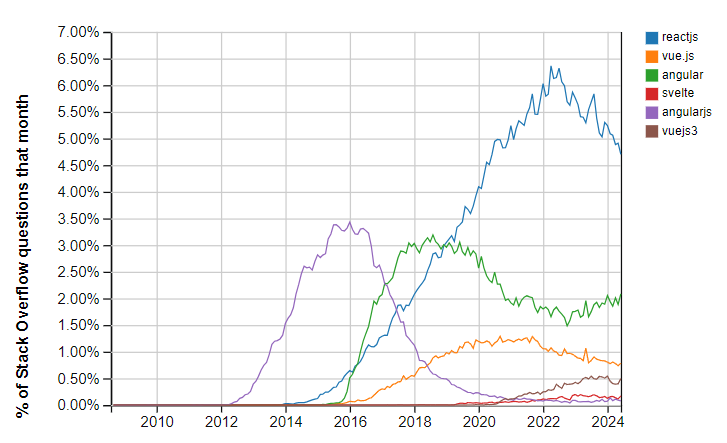
\includegraphics[width=.8\textwidth]{fetrends}
  \caption{Stackoverflow Fragen Frontend-Frameworks.}
  \label{fig:fetrends}
  \vspace{-0.3cm}
  \begin{center}
    \footnotesize Quelle: \cite{SOTrend}
  \end{center}
\end{figure}

\Cref{fig:fetrends} zeigt den Verlauf der Fragen zu Webtechnologien auf Stackoverflow,
einer sehr bekannten Plattform für Programmierfragen, über die relevanten Jahre.
Die Grafik bietet zwar keinen umfassenden Einblick in die Nutzung von Frameworks,
liefert jedoch eine grobe Orientierung darüber, welche Technologien Entwickler auch privat verwenden und somit bevorzugen.
Von der Anzahl der Fragen kann man auf die Relevanz der jeweiligen Technologien schließen.

\subsubsection{Vue}
Vue.js wurde 2014 von Evan You entwickelt und ist das jüngste der 3 Frameworks. \cite{AmD}
Es basiert auf der Idee einer \ac{SPA}, also einer Anwendung, die nur eine Seite lädt und dann dynamisch aktualisiert. \cite{BStack}
Der Vorteil an einer solchen \ac{WebApp} ist, dass sie schneller und flüssiger läuft,
da nicht bei jedem Klick die Seite neu geladen werden muss.
Vue wurde entwickelt, um die besten Teilaspekte von Angular zu übernehmen und gleichzeitig die Komplexität zu reduzieren.

Die neueste Version, Vue 3,
wurde 2020 veröffentlicht und bringt signifikante Verbesserungen und neue Funktionen mit sich. \cite{vue}
Zudem unterstützt Vue 3 die TypeScript-Integration besser, was die Typisierung und Wartung des Codes erleichtert.
\ac{TS} ist eine Programmiersprache, die auf \ac{JS} aufbaut und zusätzliche Funktionen wie Typisierung und Klassen bietet. \cite{ts}
Somit wird der Code sicherer und einfacher zu warten.

\Cref{fig:fetrends} lässt darauf schließen,
dass Vue mit Vue.js und Vue3 im Vergleich zu Angular und React weniger populär ist.
Dennoch ist es eindeutig auf Platz 3.
Zu erkennen ist ein Abfall der Fragen von VueJS und ein Anstieg von Vue 3, was den Versionswechsel verdeutlicht.
Dieser zieht sich aber eher in die Länge und geht langsam voran.

Eines der Vorteile von Vue ist, dass es eine sehr kurze Lernkurve hat. \cite{Dev}
Im Vergleich zu anderen Frameworks wie Angular,
ist Vue sehr anfängerfreundlich und benötigt nicht viele Vorkenntnisse.
Trotzdem ist es sehr leistungsstark und kann auch für größere Projekte verwendet werden.
Außerdem ist Vue sehr klein und verhindert somit, dass die Seite lange zum Laden benötigt.

Ein schwerwiegender Nachteil ist jedoch, dass es im Vergleich zu anderen Frameworks weniger Support und weniger Entwickler gibt, wie bereits aus \Cref{fig:fetrends} entnommen. \cite{BStack}
So kann es dazu führen, dass die Unterstützung von älteren Versionen fehlt oder weniger Erweiterungen verfügbar sind.
Das kann dazu führen, dass manche Funktionen selbst entwickelt werden müssen, was Zeit und Geld kostet.
Zudem fehlt im Vergleich zu Angular und React die Unterstützung von großen Unternehmen, was die Verbreitung und Weiterentwicklung einschränkt.

\subsubsection{Angular}

In Bezug auf Angular und AngularJS zeigt \Cref{fig:fetrends} eine mittlere Beliebtheit.
Während AngularJS nach seiner Veröffentlichung große Aufmerksamkeit erregte,
insbesondere aufgrund seiner revolutionären Ansätze,
wurde der Nachfolger Angular ab 2019 von React überholt und ist seither nicht mehr die beliebteste Wahl.
Der Übergang von AngularJS zu Angular erfolgte jedoch schneller als der Wechsel von Vue zu Vue 3.
Seit 2023 ist ein Anstieg der Anzahl an Fragen zu Angular zu beobachten,
was auf ein wieder wachsendes Interesse hindeutet.

Angular wurde von Google entwickelt und basiert auf \ac{TS}. \cite{NG}
Dabei ist es ein muss, \ac{TS} zu verwenden, da Angular kein JavaScript unterstützt.
Meist werden auch \ac{SPA}s mit Angular entwickelt werden, es ist jedoch auch möglich, mehrseitige Anwendungen zu erstellen.

Ein großer Vorteil von Angular ist, dass es sehr Zukunftssicher ist. \cite{BStack}
Dies kommt dadurch Zustande, da Google hinter dem Framework steht und es ständig weiterentwickelt.
Auch die Dokumentation ist sehr umfangreich und gut strukturiert, was die Einarbeitung erleichtert. \cite{NG}
Es eignet sich perfekt für große Projekt, da die Projektstruktur konsistenz und lesbarkeit fördert

Ein Nachteil ist jedoch, dass Angular sehr komplex ist und eine lange Einarbeitungszeit benötigt. \cite{BStack}
Dadurch ist es weniger für Anfänger geeignet und benötigt mehr Vorkenntnisse.
Auch die Ladezeit einer Seite ist länger, da Angular sehr groß ist und viele Funktionen mitbringt.
Bei großen \ac{WebApp}s spielt das weniger eine Rolle, aber bei kleinen \ac{WebApp}s ist es von Nachteil.

\subsubsection{React}

Wie in \Cref{fig:fetrends} erkennbar, hat sich React seit seiner Einführung als besonders beliebt erwiesen.
Die stetig wachsende Anzahl der Fragen deutet auf eine wachsende Nutzerbasis hin.
Der Höhepunkt der Beliebtheit von React war 2022, seitdem fällt die Anzahl der Fragen.

React wurde 2013 von Facebook entwickelt und gehört seither zu den beliebtesten Frontend-Frameworks. \cite{BStack}
Wie Vue und Angular ist auch React für \ac{SPA}s geeignet und verwendet ein System, in dem Komponenten wiederverwendet werden können.
Ahnlich wie Vue3 kann React auch mit \ac{TS} verwendet werden.\cite{RCT}

Ein Vorteil von React ist die relativ einfache Lernkurve. \cite{BStack}
Zudem profitieren Entwickler von der großen Community und den zahlreichen Erweiterungen,
die viele Funktionen bereits vorgefertigt anbieten,
sodass sie nicht neu programmiert werden müssen.
Damit einher geht auch das React Ökosystem, zudem auch React-Native gehört und es ermöglicht,
auch mobile Apps zu entwickeln und somit den Code zu teilen. \cite{RCTN}

Mit dem Vorteil der Größe folgt jedoch auch ein Nachteil. \cite{BStack}
Durch die Größe und Beliebtheit von React ist das Tempo der Weiterentwicklung sehr hoch,
was Entwickler zwingt, sich ständig mit neuen Konzepten auseinanderzusetzen.
Zudem verwendet React \ac{JSX}, ein spezielles Format, um \ac{HTML} in \ac{JS} zu schreiben. \cite{JSX}
Für Anfänger kann \ac{JSX} ungewohnt sein und eine gewisse Einarbeitungszeit erfordern.

\subsection{Backend-Technologien im Vergleich: Express, Springboot und Django}

Nachdem wir uns mit den Frontend-Technologien beschäftigt haben, werfen wir nun einen Blick auf die Backend-Technologien.
Dabei werden wir uns Express, Springboot und Django genauer ansehen.

16.982.234 Unternehmen nutzen laut enlyft.com Software Frameworks -
Darunter auch die Vorgestellten. \cite{eft}
Für Express fand enlyft.com 119.736 Unternehmen, für Django 37.230 und für Spring nur 138.
Die Zahlen zeigen, dass Express und Django deutlich beliebter sind als Spring.
Natürlich beziehen sich diese Zahlen nur auf eine begrenzte Anzahl von Unternehmen und sind nicht repräsentativ.
Dennoch geben sie einen groben Überblick über die Beliebtheit der Frameworks aus unternehmerischer Sicht.

\subsubsection{Express}

Wie bereits erwähnt, kann \ac{JS} auch serverseitig verwendet werden.
Dies wird durch die Nutzung von Node.js ermöglicht, wodurch \ac{JS} auch außerhalb des Browsers eingesetzt werden kann. \cite{MED}
Express ist ein populäres Framework, das auf Node.js aufbaut.

Express zeichnet sich besonders durch seine Einfachheit und Benutzerfreundlichkeit aus,
was es ideal für schnelle und unkomplizierte Lösungen macht. \cite{EiA}

Ein großer Vorteil von \ac{JS} ist,
dass Entwickler sowohl das Frontend als auch das Backend in derselben Sprache entwickeln können,
ohne eine neue Sprache erlernen zu müssen.
\ac{JS} ist jedoch eine untypisierte Sprache.
Fehler können oft erst zur Laufzeit entdeckt werden, was im Backendbereich,
wo Sicherheit und Stabilität von großer Bedeutung sind, problematisch sein kann.
\ac{TS} bietet hier eine Lösung, indem es Typisierung einführt, von welcher Express profitieren kann. \cite{EX}

Allerdings bringt die Leichtgewichtigkeit und Flexibilität von Express auch einige Nachteile mit sich. \cite{EiA}
Es fehlen integrierte Funktionen, die andere, umfangreichere Frameworks bieten,
wie z.B. Datenbankintegration, Sicherheitsfunktionen oder Authentifizierungsmechanismen.
Diese müssen in Express durch zusätzliche Module ergänzt werden,
was zusätzlichen Zeitaufwand erfordert und eine sorgfältige Verwaltung der Abhängigkeiten notwendig macht.

\subsubsection{Springboot}

Spring Boot ist ein leistungsstarkes Framework für die Backend Entwicklung in Java,
das auf dem bewährten Spring Framework basiert. \cite{MED}
Es vereinfacht die Entwicklung erheblich, indem es den Ansatz “Convention over Configuration” verfolgt.
Das bedeutet, dass viele Konfigurationen automatisch übernommen werden,
was den typischen Boilerplate-Code durch Java reduziert und den Entwicklern ermöglicht,
sich auf die wesentlichen Teile ihrer Anwendung zu konzentrieren.

Viele wichtige Funktionen, wie die Integration von Datenbanken oder Sicherheitsfunktionen,
werden von Spring Boot direkt unterstützt. \cite{SPR}
Dies bedeutet, dass Entwickler nicht auf Drittanbieter-Bibliotheken zurückgreifen müssen,
um grundlegende Funktionalitäten zu implementieren.

Ein Beispiel dafür, wie Spring Boot die Entwicklung erleichtert, ist die automatische Konvertierung von Java-Klassen in \ac{JSON}.
So können Entwickler einfach Objekte erstellen und diese direkt an den Client senden, ohne sich um die Konvertierung kümmern zu müssen.

Solche Funktionen machen Spring Boot beliebt, aber diese vermeindliche Magie hat auch Nachteile. \cite{EiA}
Die Automatisierungen können dazu führen, dass Entwickler nicht verstehen, was im Hintergrund passiert.
Somit steigt auch die Lernkurve, da es sehr aufwendig sein kann, sich in die genauen Funktionsweisen einzuarbeiten.
Darüber hinaus kann die Komplexität von Spring Boot bei kleineren Projekten zu zusätzlicher Rechneleistung führen, die genutzt, aber nicht benötigt wird.

\subsubsection{Django}

Django basiert auf Python und zeichnet sich, ähnlich wie Spring, dadurch aus,
dass es alle notwendigen Komponenten für die Entwicklung einer Webanwendung bereits integriert hat.
Dies vereinfacht den Entwicklungsprozess erheblich. \cite{MED}

Ein besonders markantes Merkmal von Django ist das automatisch generierte Admin-Interface.
Dieses erleichtert die Verwaltung von Datenbanken erheblich und spart Entwicklern viel Zeit und Arbeit,
da sie keine eigene Verwaltungsoberfläche entwickeln müssen. \cite{DJO}

Darüber hinaus bietet Django standardmäßig umfangreiche Sicherheitsmechanismen,
wie z.B. den Schutz gegen \ac{SQL}-Injections, ein Angriff auf die Datenbank.
Dadurch können Entwickler sichere Anwendungen erstellen,
ohne sich um viele der typischen Sicherheitslücken kümmern zu müssen.

Ein Nachteil von Django ist jedoch,
dass das Framework sehr strikt aufgebaut ist und wenig Flexibilität bietet. \cite{MED}
Diese Striktheit kann in einigen Projekten als Einschränkung empfunden werden,
insbesondere wenn besondere Anpassungen erforderlich sind.
Darüber hinaus hat Django eine eher steile Lernkurve, insbesondere für Entwickler, die noch nicht mit Python vertraut sind.

\subsection{Wie arbeiten Backend und Frontend zusammen?}

Es gibt mehrere Möglichkeiten, wie das Backend mit dem Frontend kommunizieren kann.
Zwei der gängigsten Methoden sind \ac{REST}-\ac{API}s und WebSocket-Server.
Beide basieren auf \ac{HTTP}, ein Protokoll, das die Kommunikation zwischen Server und Client ermöglicht.
Während \ac{REST}-\ac{API}s in den meisten klassischen \ac{WebApp}s für den Datenaustausch verwendet werden,
sind WebSockets besonders für Echtzeitanwendungen von großer Bedeutung. \cite{ReSock}

\begin{figure}
  \centering
  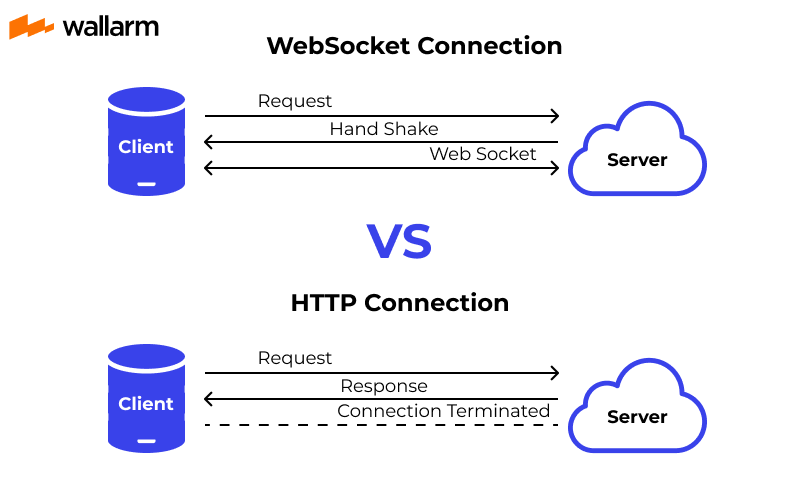
\includegraphics[width=.8\textwidth]{communication}
  \caption{REST-APIs vs. WebSockets}
  \label{fig:communication}
  \vspace{-0.3cm}
  \begin{center}
    \footnotesize Quelle: \cite{WebCon}
  \end{center}
\end{figure}

\Cref{fig:communication} zeigt den grundlegenden Unterschied zwischen \ac{REST}-\ac{API}s (unten) und WebSockets (oben).

\ac{REST}-\ac{API}s basieren auf dem klassischen Anfrage-Antwort-Modell.
Das Frontend sendet eine \ac{HTTP}-Anfrage an das Backend und erhält eine Antwort in Form von \ac{JSON} oder einem anderen Format zurück.

WebSockets hingegen ermöglichen eine Echtzeit-Kommunikation.
Sobald eine Verbindung zwischen dem Client (Frontend) und dem Server (Backend) hergestellt ist,
können beide Seiten kontinuierlich Nachrichten senden und empfangen, ohne die Notwendigkeit, eine neue Anfrage zu stellen.
Dies ist besonders nützlich für Anwendungen wie Chats oder Multiplayer-Games.

\section{Die GLS Quiz App}

Nachdem alle nötigen Grundlagen geschaffen sind, befassen wir uns im folgenden Abschnitt weiter mit der GLS Quiz App.
Wir lernen sie näher kennen, zeigen ihre Probleme auf und kombinieren das bereits gesammelte Wissen in einer Nutzwertanalyse.

\subsection{Ist-Zustand der App}

Die GLS Quiz App bietet mehrere Modi und eine Punktzahlberechnung,
die von der Antwortzeit abhängt. \cite{GLSQ}
Für jede Frage gibt es mehrere Antwortmöglichkeiten,
die zufällig angezeigt werden.
Auch die Fragen werden dabei in zufälliger Reihenfolge gestellt.
Der Nutzer erhält maximal 100 Punkte pro Frage,
die bei schneller Antwort (innerhalb von 20 Sekunden) vollständig gewertet wird,
wobei die Punkte mit ablaufender Zeit (−1 Punkt pro Sekunde) sinken.
Es gibt verschiedene Modi, darunter das Zustellungsquiz,
das Allgemeine Quiz und den Rapid Modus, bei dem die Punktabzüge nach 5 Sekunden beginnen.
Im folgenden wird sich nur mit dem Zustellungsquiz beschäftigt.

\begin{figure}
  \centering
  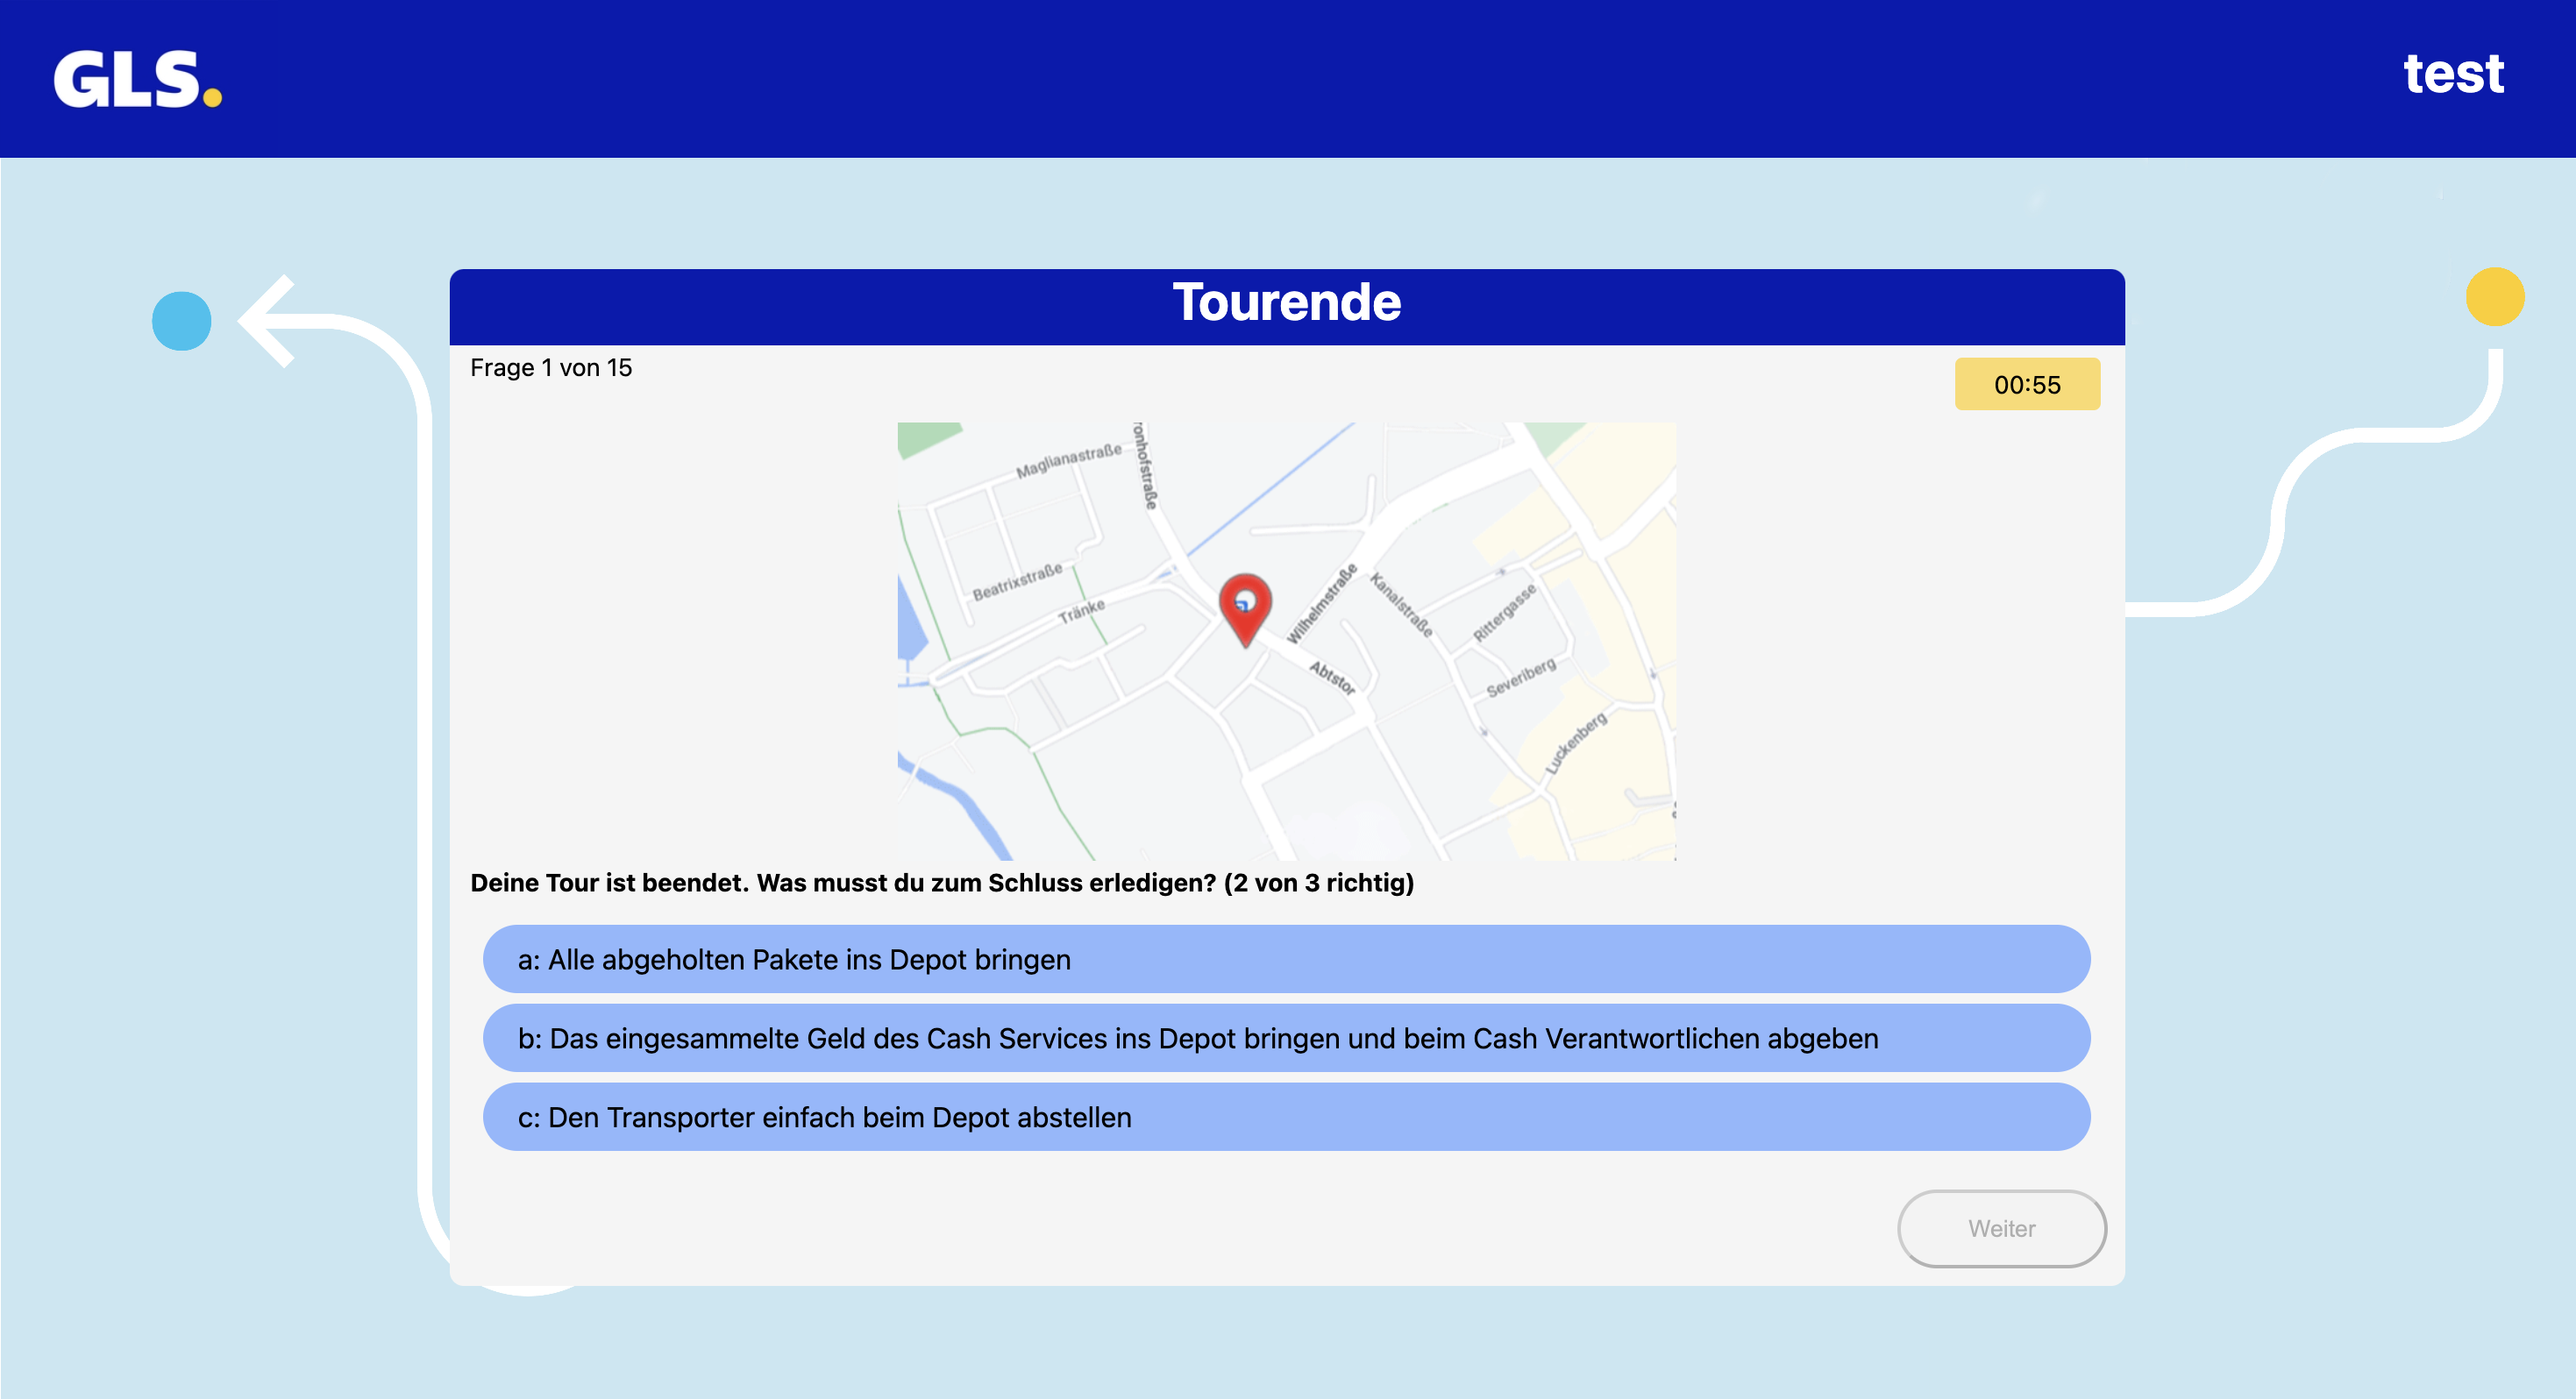
\includegraphics[width=.8\textwidth]{gls-trainee}
  \caption{GLS Zustellquiz}
  \label{fig:gls-trainee}
\end{figure}

Nach dem Beantworten der Fragen zeigt die App am Ende eine Auswertung.
Diese enthält eine Auflistung der erreichten Punkte, welche Antworten gewählt wurden, und welche korrekt gewesen wären.
Je nach Punktestand gibt es ein angepasstes Feedback, z.B. “Du musst noch ein bisschen üben…”.
Zudem existiert eine Bestenliste pro Modus.

Die App nutzt reines \ac{HTML}, \ac{CSS} und \ac{JS} im Frontend und speichert die Bestenliste in Amazon AWS DynamoDB. \cite{GLSQS}
Änderungen und Aktualisierungen in der \ac{WebApp} erfolgen über den Austausch von \ac{HTML}-Elementen durch \ac{JS}.
Die Fragen sind in einer \ac{JS}-Datei hinterlegt und einsehbar.
Ein Teil der App-Komponenten wurde modularisiert,
doch es besteht weiterhin doppelter Code und die Dateien sind teils sehr groß.

\subsection{Ursprüngliches Konzept}

Wie bereits in der Einleitung angerissen basierte das ursprüngliche Konzept der App auf einem analogen Quiz,
das einen Zustelltag simulierte.
In dieser Version mussten die Nutzer eine feste Route mit verschiedenen Stopps abarbeiten.
Die Fragen waren an eine feste Position auf einer Karte gebunden und hatten Namen wie „Stopp: David“,
um eine reale Zustellsituation nachzubilden.
Die Reihenfolge der Fragen war nicht zufällig, sondern folgte der Route, ähnlich wie bei einer Auslieferung.

Ziel der GLS-Quiz App war es, die analoge Version zu digitalisieren.

\subsection{Problem bei der Umsetzbarkeit des ursprünglichen Konzepts}

Das Hauptproblem bei der Umsetzung war die Implementierung einer interaktiven Karte,
die auswählbare Stopps für den Nutzer bietet.
Dieses Features erwies sich als schwierig und konnte nicht einfach mit \ac{HTML}, \ac{CSS} und \ac{JS} realisiert werden.

\subsection{Konzeptentwicklung zur Bewältigung der Herausforderungen}

Die Hauptkriterien für die Neuentwicklung der App sind:
\begin{itemize}
  \item \textbf{Strukturierter Aufbau:} Ein strukturiertes Komponentensystem soll die Weiterentwicklung und Wiederverwendung von Code fördern.
  \item \textbf{Sicherheit der Fragen:} Die Fragen sollen im Quelltext nicht einsehbar sein, um das Schummeln mit den Lösungen zu verhindern.
  \item \textbf{Einfache Lernkurve:} Die App soll eine einfache Lernkurve haben, damit neue Studenten schnell in die Entwicklung einsteigen können.
  \item \textbf{Einfache Map-Integration:} Eine einfache Integration von Kartenfunktionen soll gewährleistet sein.
  \item \textbf{Leichtgewichtigkeit:} Die App soll leichtgewichtig sein, weil sie nur einen begrenzten Funktionsumfang hat.
\end{itemize}

Um die Herausforderungen zu lösen, wird eine Trennung zwischen Frontend und Backend eingeführt.
So sollen die Fragen im Backend verborgen und dynamisch geladen werden.
Somit ist die Sicherheit der Fragen für alle Kombination gewährleistet.
Zur besseren Strukturierung des Codes sollen Frameworks verwendet werden, die einen modularen Aufbau und wiederverwendbare Komponenten ermöglichen.
Im Frontend folgt zusätzlich die Integration von Karten zur Simulation der Zustellrouten.
Dafür werden die jeweiligen Optionen der Frameworks für die Integration von Google Maps basierend auf der Einfachheit der Integration bepunktet,
siehe @angular/google-maps \cite{ngMaps}, @react-google-maps/api \cite{rctMaps} und @fawmi/vue-google-maps \cite{vueMaps}.
Alle anderen Kriterien werden mit dem Wissen aus dem \hyperref[sec:tec-überblick]{\textit{Technologieüberblick}} bewertet.

\begin{table}[h!]
  \centering
  \caption{Nutzwertanalyse der Frontend-Frameworks}
  \label{tab:nutz-frontend}
  \begin{tabular}{@{}lcccc@{}}
    \toprule
    \textbf{Kriterien} & \textbf{Gewichtung} & \textbf{Vue} & \textbf{React} & \textbf{Angular} \\ \midrule
    \textbf{Lernkurve einfach} & 35\% & 4 & 3 & 1 \\ \midrule
    \textbf{strukturierter Aufbau} & 25\% & 3 & 3 & 4 \\ \midrule
    \textbf{Maps Integration} & 20\% & 3 & 2 & 4 \\ \midrule
    \textbf{Leichtgewichtig} & 20\% & 4 & 3 & 2 \\ \midrule
    \textbf{Summe} & 100\% & 3.55 & 2.8 & 2.55 \\ \bottomrule
  \end{tabular}
\end{table}

\begin{table}[h!]
  \centering
  \caption{Nutzwertanalyse der Backend-Frameworks}
  \label{tab:nutz-backend}
  \begin{tabular}{@{}lcccc@{}}
    \toprule
    \textbf{Kriterien} & \textbf{Gewichtung} & \textbf{Spring} & \textbf{Express} & \textbf{Django} \\ \midrule
    \textbf{Lernkurve einfach} & 35\% & 3 & 4 & 2 \\ \midrule
    \textbf{strukturierter Aufbau} & 25\% & 4 & 3 & 3 \\ \midrule
    \textbf{Leichtgewichtig} & 20\% & 2 & 4 & 3 \\ \midrule
    \textbf{Summe} & 80\% & 2.45 & 2.95 & 2.05 \\ \bottomrule
  \end{tabular}
\end{table}

Die beiden Tabellen \ref{tab:nutz-frontend} und \ref{tab:nutz-backend} zeigen die Nutzwertanalyse der Frontend- und Backend-Frameworks.
Anhand der Gewichtung der Kriterien wird deutlich,
dass Angular und Django die schlechtesten Werte erzielen und somit nicht für eine Umsetzung geeignet sind.
\newpage

\section{Test-Implementierung}

Um das Verständnis zu vertiefen und die Bewertung der Technologien im Bezug auf die GLS-Quiz App zu erleichtern,
wird in diesem Abschnitt ein Demo Projekt vorgestellt.

Das Hauptziel besteht darin,
einen Überblick über alle vorgestellten Frontend- und Backend-Technologien zu schaffen,
um später die bestmögliche Kombination für die finale Lösung zu ermitteln.
Dazu wird ein Prototyp entwickelt, der mit allen bereits vorgestellten Frontend- und Backend-Technologien realisiert wird,
sowohl auf der Backend-Seite (Spring Boot, Express, Django) als auch auf der Frontend-Seite (Vue, Angular, React).

\subsection{Das Demo Projekt}

Das Demo-Projekt ist eine simple Fragen-App und simuliert damit auf einer sehr einfachen Ebene die GLS-Quiz App.
Die App ist in zwei Hauptteile unterteilt: Frontend und Backend, wie in dem Abschnitt \hyperref[sec:moderne-webtechnologien]{\textit{Überblick über moderne Webtechnologien}} beschrieben.

Die Fragen-App stellt dem Nutzer nacheinander verschiedene Fragen,
die jeweils mehrere Antwortmöglichkeiten bieten \textit{(a, b, c)}.
Jede Frage hat genau eine richtige Antwort.
Der Nutzer kann eine Antwort auswählen und muss diese anschließend bestätigen.
Nach der Bestätigung erhält der Nutzer eine Rückmeldung,
ob seine Antwort richtig oder falsch war.
Es ist sicherzustellen, dass der Nutzer nicht durch Einsicht in den Quelltext der App die korrekten Antworten herausfinden kann.

Das Frontend ist ausschließlich für die visuelle Darstellung der \ac{WebApp} zuständig.
Es zeigt die Fragen, die Antwortmöglichkeiten und das Ergebnis der Beantwortung an.

Das Backend fungiert als \ac{REST}-\ac{API} und ist verantwortlich für die Bereitstellung der Fragen und die Überprüfung der Antworten.
Das Thema Datenbank ist zu vernachlässigen.
Stattdessen soll das Backend auf eine einfache Methode zurückgreifen, wie zum Beispiel die Verwendung einer einzelnen Datei.

\subsection{Umsetzung}

Das gesamte Projekt mit zusätzlichen Informationen und Code ist auf GitHub unter folgendem Link verfügbar: https://github.com/hypeAlive/fallstudie-impl. \cite{fImpl}
Für jedes Backend und Frontend ist die wichtigste Code-Datei im \hyperref[sec:anhang]{\textit{Anhang}} enthalten.
Im Backend handelt es sich um die Routendefinition und im Frontend um die QuestionComponent.

\subsubsection{Frontend}

Für das Design kommt Tailwind\ac{CSS} zusammen mit der Bibliothek daisyUI zum Einsatz,
um das Layout und die Komponenten zu gestalten.

Die Hauptkomponente ist immer sichtbar und enthält sämtliche Routen.
Direkt beim Laden der Seite wird der Typ des Backends vom Server abgefragt.
Basierend auf dieser Information wird dann das entsprechende Backend-Bild angezeigt,
das zusammen mit einem Bild des Frontends in der Oberfläche eingebettet wird.

Die Startseite der Anwendung (im Code bezeichnet als HomeComponent),
die unter der Route / erreichbar ist, zeigt einen Button mit der Aufschrift “Start” an.
Durch einen Klick auf diesen Button wird der Benutzer auf die Route /question weitergeleitet,
die das eigentliche Quiz beinhaltet.

Die Quiz-Seite (im Code bezeichnet als QuestionComponent) fragt beim ersten Laden alle verfügbaren \ac{ID}s an Fragen vom Backend ab.
Sobald die \ac{ID}s verfügbar sind,
wählt das Frontend zufällig eine \ac{ID} aus und fragt die dazugehörige Frage und deren Antwortmöglichkeiten vom Backend ab.
Diese Informationen werden dann auf der Seite angezeigt.

\begin{figure}
  \centering
  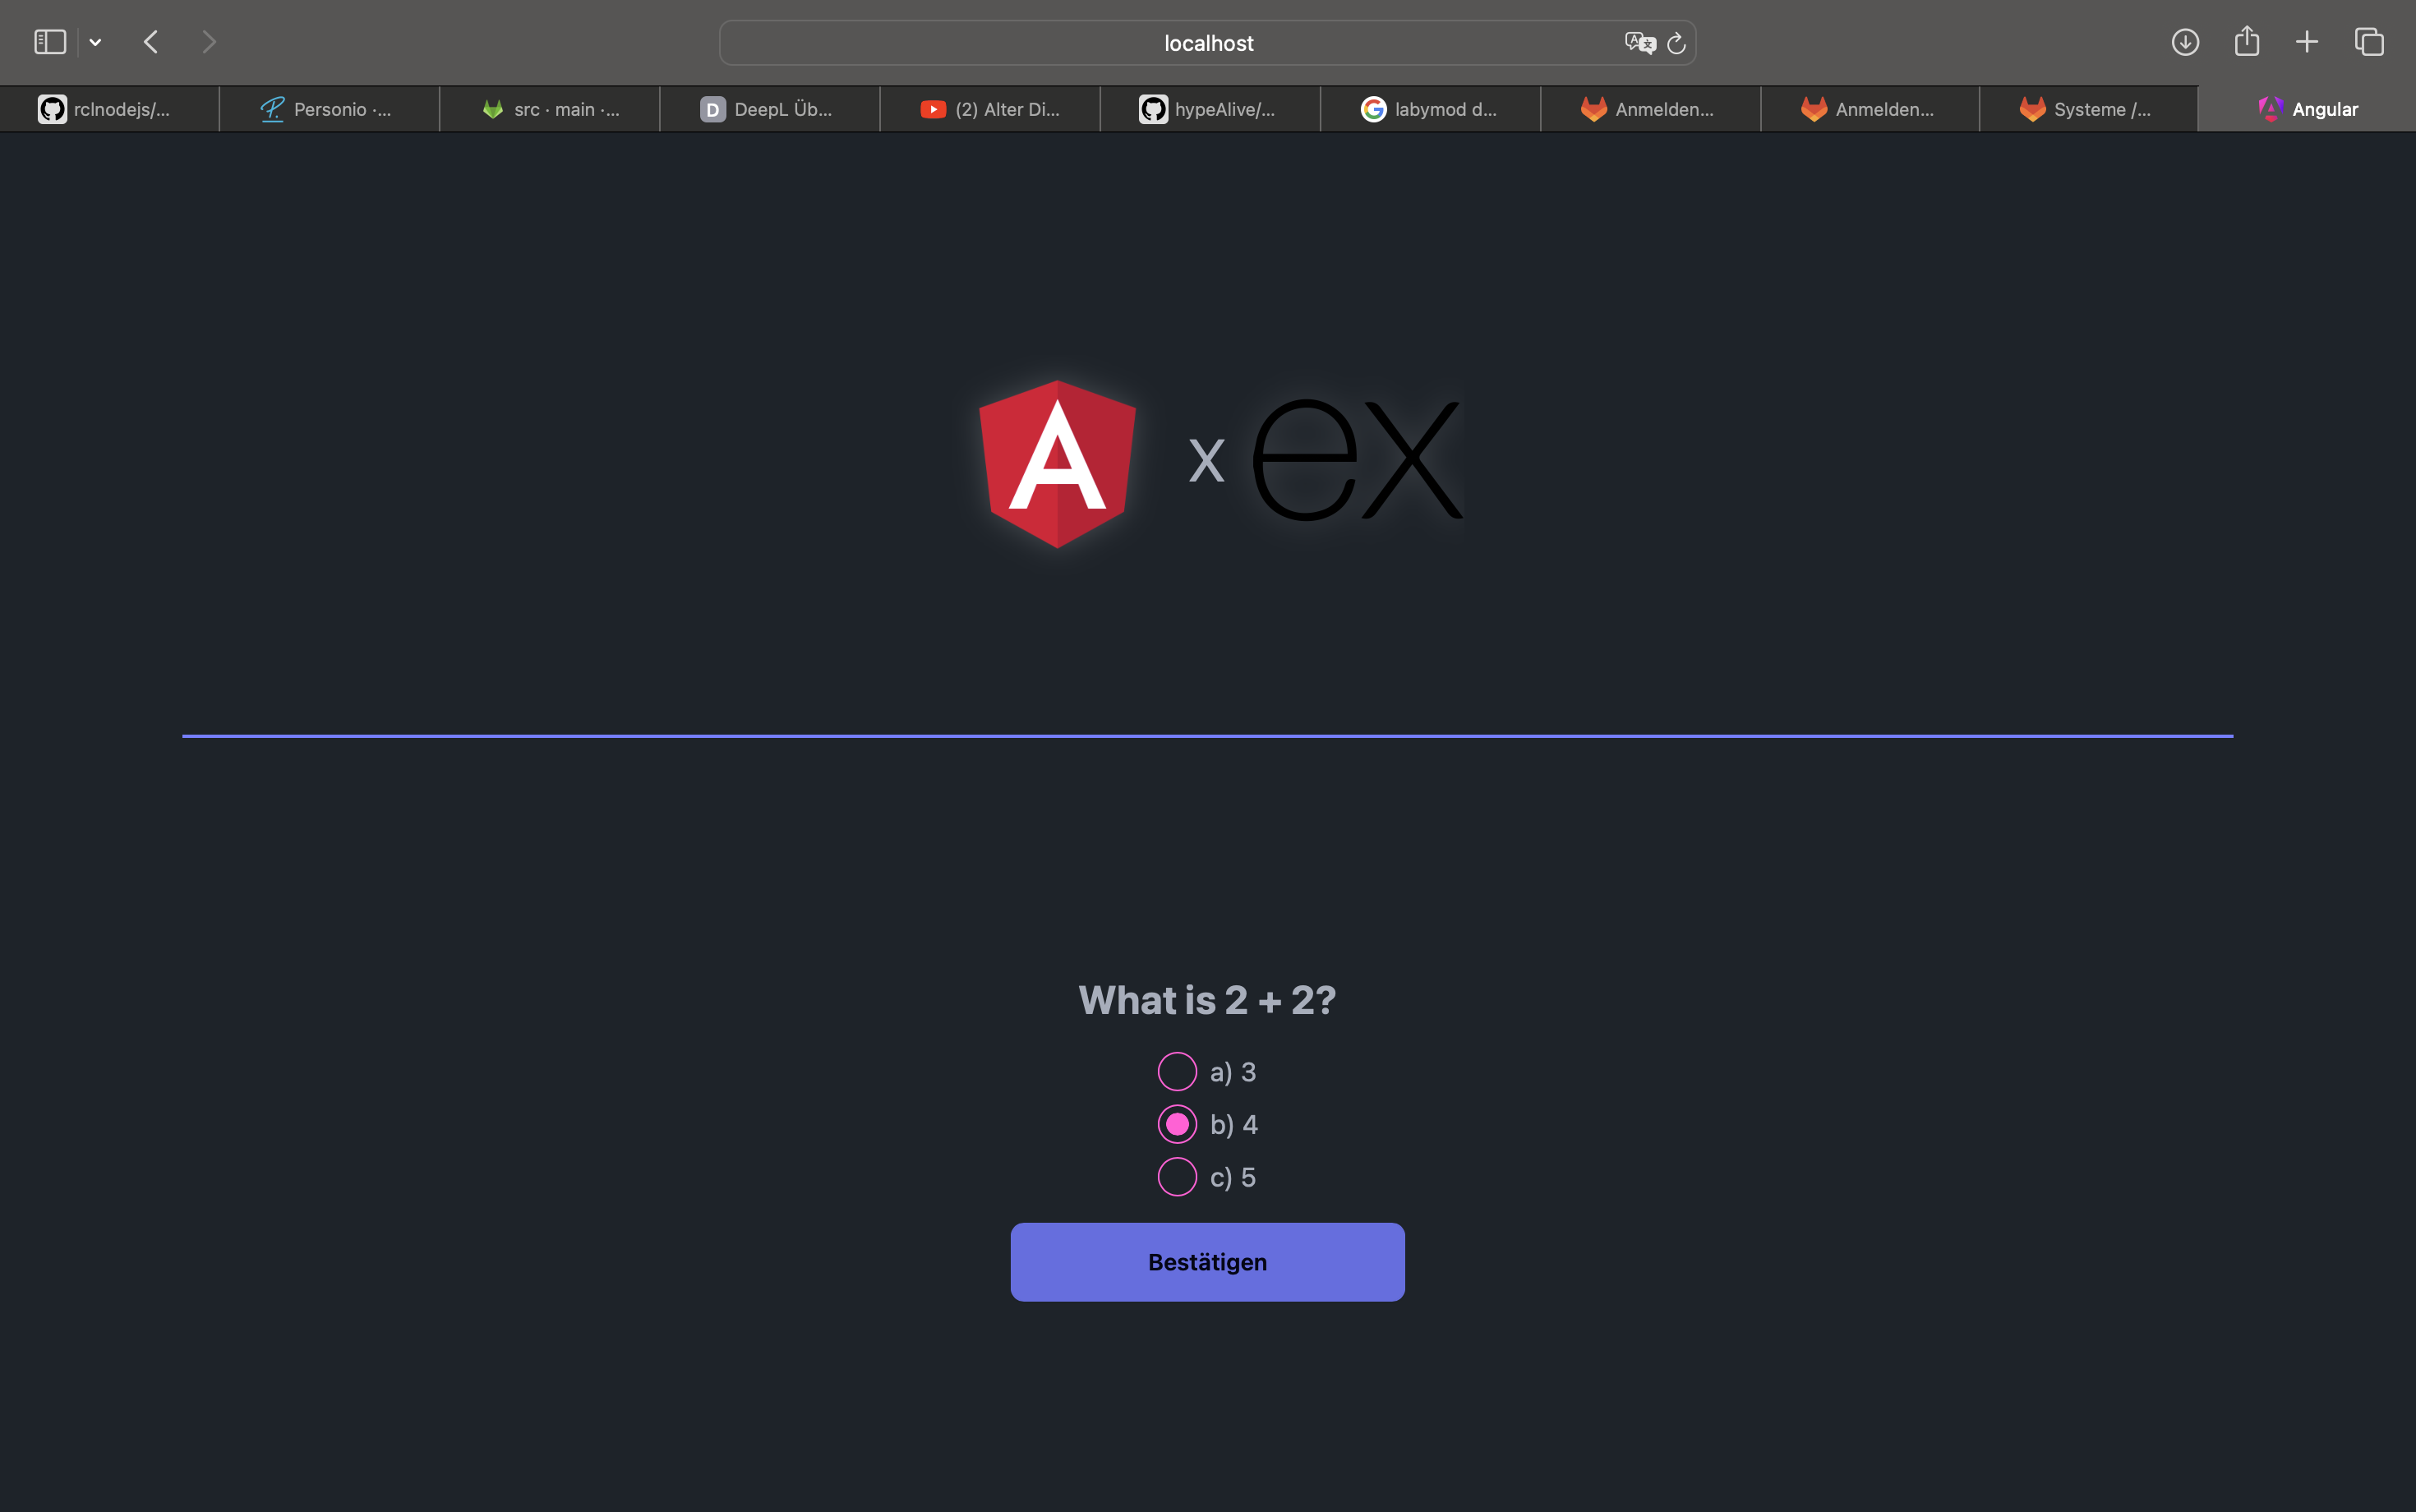
\includegraphics[width=.8\textwidth]{question-component}
  \caption{Route \textit{/question} mit Angular und Express.}
  \label{fig:question-component}
\end{figure}

Zusätzlich dazu enthält diese Seite einen Button,
der je nach Zustand der Anwendung unterschiedliche Funktionen erfüllt.
Wenn eine Frage geladen und angezeigt wird, ermöglicht er dem Nutzer,
seine ausgewählte Antwort zu bestätigen.
Diese Antwort wird an das Backend gesendet, wo sie auf Richtigkeit geprüft wird.
Anschließend erhält der Nutzer eine Rückmeldung, ob seine Antwort korrekt war.
Nach dieser Überprüfung ändert sich die Funktion des Buttons, und ermöglicht es die nächste Frage zu laden.

\subsubsection{Backend}

Das Backend sendet und empfängt \ac{JSON}-Daten.
Außderdem hat es eine simulierte Datenbank, die in Form einer \ac{JSON}-Datei vorliegt.
Diese Datei wird beim Start des Backends einmalig geladen.

Backends sind durch Routen definiert, die bestimmte Endpunkte bereitstellen.
Diese Endpunkte erlauben es dem Frontend, verschiedene Anfragen an das Backend zu senden, etwa um Fragen aus der Datenbank zu laden oder um Antworten zu überprüfen.
Die genauen Routen und ihre Definitionen sind im Anhang zu finden.

\subsection{Ergebnisse und erlangtes Wissen}

Folgende Tabellen fassen die wichtigsten Erkenntnisse aus der Implementierung zusammen:

\begin{table}[h!]
  \centering
  \caption{Vergleich der Backend-Frameworks}
  \begin{tabular}{@{}llll@{}}
    \toprule
    \textbf{Kriterium}            & \textbf{Django}                                             & \textbf{Express}                                           & \textbf{Spring}                                             \\ \midrule
    \textbf{Zeilen Code (LoC)}    & 165                                                        & 135                                                        & 173                                                        \\ \midrule
    \textbf{Vorteile}             & \begin{tabular}[c]{@{}l@{}}+ Übersichtlich: \\ \texttt{urls.py} \\ + Admin-Interface \\ automatisch generiert\end{tabular} & \begin{tabular}[c]{@{}l@{}}+ Einfache, \\ übersichtliche \\ Struktur\\ + Leicht zu verstehen\end{tabular} & \begin{tabular}[c]{@{}l@{}}+ Schnelle \\ Einrichtung\\ + Automatische \\ Konvertierung von \\ Java-Klassen zu JSON\end{tabular} \\ \midrule
    \textbf{Nachteile}            & \begin{tabular}[c]{@{}l@{}}- Aufwendige \\ Einrichtung\\ - Python anders \\ als im Frontend\end{tabular} & \begin{tabular}[c]{@{}l@{}}- Alles manuell \\ schreiben\\ - Mit TypeScript \\ aufwendiger\end{tabular} & \begin{tabular}[c]{@{}l@{}}- Weniger \\ übersichtliche Routen\\ - Neue Sprache \\ im Vergleich zum \\ Frontend\end{tabular} \\ \bottomrule
  \end{tabular}
\end{table}

\begin{table}[h!]
  \centering
  \caption{Vergleich der Frontend-Frameworks}
  \begin{tabular}{@{}llll@{}}
    \toprule
    \textbf{Kriterium}            & \textbf{Angular}                                            & \textbf{React}                                             & \textbf{Vue}                                               \\ \midrule
    \textbf{Zeilen Code (LoC)}    & 213                                                        & 190                                                        & 176                                                        \\ \midrule
    \textbf{Vorteile}             & \begin{tabular}[c]{@{}l@{}}+ Klare Trennung: \\ HTML, CSS, TS\\ + Einfacher \\ HttpClient\end{tabular} & \begin{tabular}[c]{@{}l@{}}+ Weniger Dateien\\ + Einstieg leicht \\ durch weniger Konzepte\end{tabular} & \begin{tabular}[c]{@{}l@{}}+ Ähnlich wie React \\ + Einfache Struktur\\ + Schneller Einstieg\end{tabular} \\ \midrule
    \textbf{Nachteile}            & \begin{tabular}[c]{@{}l@{}}- Viele Konzepte\\ für den Einstieg\end{tabular} & \begin{tabular}[c]{@{}l@{}}- JSX ungewohnt\\ - Externe Library \\ für Anfragen nötig\end{tabular} & \begin{tabular}[c]{@{}l@{}}- Kombination \\ von .vue Dateien \\ ungewohnt\\ - Externe Library \\ für Anfragen nötig\end{tabular} \\ \bottomrule
  \end{tabular}
\end{table}

Zusammenfassend haben sich einige Vor- und Nachteile der verschiedenen Frameworks bestätigt.
Zum Beispiel punktet Express durch seine Einfachheit und Flexibilität, während Django und Spring durch automatische Features überzeugen.

Auf der Frontend-Seite hat sich gezeigt, dass Angular durch seine klare Trennung von \ac{HTML}, \ac{CSS} und \ac{TS} gut strukturiert,
jedoch schwieriger zu erlernen ist.
React und Vue bieten einen einfacheren Einstieg.
Vue kombiniert dabei die Vorteile von React und Angular.

Der wichtigste Erkenntnisgewinn aus der Implementierung ist jedoch,
dass die Wahl der Kombination von Frontend- und Backend-Frameworks nicht entscheidend für den Erfolg der Implementierung ist.
Die Kommunikation zwischen den beiden Schichten erfolgt grundsätzlich auf ähnliche Weise,
und es liegt eher an den individuellen Anforderungen und Präferenzen des Entwicklers, welche Technologien gewählt werden.

\section{Schlussfolgerung und Ausblick}

In dieser Fallstudie wurde ein umfassender Überblick über moderne Webtechnologien gegeben
und deren Eignung in Bezug auf die GLS Quiz App analysiert.
Die Untersuchung umfasste sowohl drei Frontend- als auch drei Backend-Frameworks,
wobei die Kriterien Lernkurve, Struktur, Integration von Karten und Leichtgewichtigkeit im Vordergrund standen.
Es wurden grundlegende Begriffe und Konzepte zur Zusammenarbeit vorgestellt, wie \ac{SPA}s, \ac{REST}-\ac{API}s und WebSockets.

Die Nutzwertanalyse zeigte, dass Vue und React im Frontend-Bereich die besten Ergebnisse erzielten,
während Angular aufgrund seiner Komplexität und steilen Lernkurve weniger geeignet erschien.
Im Backend-Bereich überzeugten Express und Spring durch ihre einfachere Lernkurve,
während Django ein Mittelmaß aller Kriterien darstellte.

Die Testimplementierung bestätigte diese Ergebnisse und zeigte,
dass die Wahl der Kombination von Frontend- und Backend-Frameworks nicht entscheidend für den Erfolg der Implementierung ist.
Vielmehr hängt der Erfolg von den spezifischen Anforderungen und Präferenzen des Entwicklers ab.
Zusätzlich wurde deutlich, dass generell jede Wahl möglich ist,
aber die Vorteile und Nachteile der jeweiligen Technologie dennoch große Auswirkungen
auf die Entwicklung und das Ergebnis haben können.

Aus den Ergebnissen der Fallstudie lässt sich ableiten,
dass Vue und Express die beste Kombination für die Entwicklung der GLS Quiz App darstellen.
Diese Kombination bietet eine gute Balance zwischen Einfachheit, Flexibilität und Leistungsfähigkeit.
Eine Option für das Frontend wäre auch React gewesen,
da React eine größere Community hat und somit mehr Ressourcen und Unterstützung bietet.
Da die GLS Quiz App jedoch einen relativ geringen Funktionsumfang hat, wiegt dieser Punkt weniger schwer.
Bezüglich des Backends punktet Express vor allem durch den Fakt,
dass es auf Node.js basiert und somit \ac{JS} sowohl im Frontend als auch im Backend verwendet werden kann.

Zukünftig sollte die Entwicklung der GLS Quiz App weiter vorangetrieben werden,
indem die gewonnenen Erkenntnisse aus dieser Fallstudie genutzt werden.
Es ist wichtig, dass, wenn das ursprüngliche Konzept umgesetzt oder die Anwendung weiterentwickelt werden soll,
auf genannte Technologien gesetzt wird.

Anhand der Entscheidung am Beispiel der GLS Quiz App wurde deutlich,
wie bei der Auswahl von Technologien vorzugehen ist.
Es zeigte sich, dass grundsätzlich viele Optionen möglich sind,
jedoch die spezifischen Anforderungen und Ziele des Projekts entscheidend sind.
Die Vor- und Nachteile der verschiedenen Technologien müssen sorgfältig abgewogen werden.
Ein minimaler Prototyp ist dabei definitiv den Zeitaufwand wert, da er hilft,
die Technologien besser zu verstehen und die richtige Wahl zu treffen.
Dies ermöglicht eine fundierte Entscheidung und trägt maßgeblich zum Erfolg des Projekts bei.

\newpage
\section{Glossar}

\begin{description}
  \item[Software:] Programme, Skripte oder Anwendungen

  \item[Webanwendung:] Anwendung, die über einen Browser erreichbar ist. Beispiele: Online-Shops, soziale Netzwerke...

  \item[Dokumentationen:] Schriftliche Anleitungen und Beschreibungen, zur Anwendung und Funktionsweise von Software.

  \item[Server und Client:] Ein Server bietet Dienste an, die ein Client nutzt.

  \item[(Boilerplate-)Code:] Code ist eine Date, gefüllt mit Anweisungen für den Computer. Boilerplate-Code sind standardisierte und wiederkehrende Codeabschnitte.

  \item[Typisierung:] Das Festlegen von Typen in Programmiersprachen. Zum Beispiel: Zahl, Zeichenkette oder Objekt.

  \item[Klassen und Objekte:] Ein Objekt ist eine Instanz einer Klasse. Eine Klassen ist eine Blaupause, die Objekte erzeugt.

  \item[Support:] Wenn eine Software weiterentwickelt wird und nicht mehr mit älteren Versionen kompatibel ist, wird der Support dieser eingestellt.

  \item[(Projekt-)Struktur:] Die Art und Weise, wie ein Projekt organisiert und aufgebaut ist.

  \item[Komponenten:] Einzelne Teile einer Anwendung, die in sich abgeschlossen sind. Sind modular, da sie unabhängig voneinander entwickelt werden können.

  \item[Quelltext (Browser):] Der einsehbare Code einer Webseite.

  \item[Routen:] Die Pfade oder URLs, die definieren, welche Daten oder Seiten bei Aufruf im Browser angezeigt werden.

\end{description}

\newpage

\section*{\centering Eigenständigkeitserklärung}

\vspace{1cm}

\noindent
Hiermit bestätige ich,
dass ich die vorliegende Arbeit selbständig verfasst habe.
Die Stellen der Arbeit, die dem Wortlaut oder dem Sinn nach anderen Werken (dazu zählen auch Internetquellen) entnommen sind,
wurden unter Angabe der Quelle kenntlich gemacht.

\vspace{3cm}

\noindent
\makebox[5cm][c]{Fulda, \today} \hfill \makebox[5cm][c]{} \\
\makebox[5cm]{\hrulefill} \hfill \makebox[5cm]{\hrulefill} \\
\makebox[5cm][c]{\textit{Ort, Datum}} \hfill \makebox[5cm][c]{\textit{Unterschrift}}

\newpage

\printbibliography

\newpage


\section{Anhang}
\label{sec:anhang}
\subsection{Implementierung}

\subsubsection{Komponenten}

\textit{\textbf{QuestionComponent} Angular} \\
\begin{lstlisting}[caption={question.component.ts}, label=qc-ng, language=typescript]
import {Component, OnInit} from '@angular/core';
import {HttpClient} from "@angular/common/http";
import {AppComponent} from "../app.component";
import {firstValueFrom} from "rxjs";
import {AnswerRes, AnswerType, QuestionHidden} from "api-types";
import {NgClass, NgForOf, NgIf, NgTemplateOutlet} from "@angular/common";
import {QuestionOption} from "api-types/dist/quiz.type";

@Component({
  selector: 'app-question',
  standalone: true,
  imports: [
    NgForOf,
    NgIf,
    NgClass,
    NgTemplateOutlet
  ],
  templateUrl: './question.component.html',
  styleUrl: './question.component.css'
})
export class QuestionComponent implements OnInit{

  private static QUESTIONS: number[] | undefined = undefined;

  protected question: QuestionHidden | undefined = undefined;
  protected selectedAnswer: AnswerType | undefined = undefined;
  protected isCorrect: boolean | undefined = undefined;
  protected isLoading: boolean = true;

  constructor(private http: HttpClient) {
  }

  ngOnInit(): void {
    if (QuestionComponent.QUESTIONS === undefined) {
      firstValueFrom<number[]>(this.http.get<number[]>(AppComponent.API_URL + '/question/ids'))
        .then(r => {
          QuestionComponent.QUESTIONS = r;
          this.requestRandomQuestions();
        })
    } else {
      this.requestRandomQuestions();
    }
  }

  protected requestRandomQuestions(): void {
    this.isLoading = true;
    this.question = undefined;
    this.selectedAnswer = undefined;
    this.isCorrect = undefined;
    firstValueFrom<QuestionHidden>(this.http.get<QuestionHidden>(AppComponent.API_URL + '/question/' + QuestionComponent.QUESTIONS![Math.floor(Math.random() * QuestionComponent.QUESTIONS!.length)]))
      .then(r => {
        this.question = r;
        this.isLoading = false;
        console.log(r);
      });
  }

  protected onOptionSelected(option: QuestionOption): void {
    this.selectedAnswer = option.type;
  }

  protected submitAnswer(): void {
    if(!this.selectedAnswer || !this.question) return;

    const checkId = this.question.id;
    this.question = undefined;
    this.isLoading = true;

    firstValueFrom<AnswerRes>(this.http.post<AnswerRes>(AppComponent.API_URL + '/question', {
      id: checkId,
      answer: this.selectedAnswer
    }))
      .then(r => {
        console.log(r);
        this.isCorrect = r.isCorrect;
        this.isLoading = false;
      });
  }
}
\end{lstlisting}

\textit{\textbf{QuestionComponent} React} \\
\begin{lstlisting}[caption={QuestionComponent.jsx}, label=qc-rc, language=javascript]
import React, { useEffect, useState } from 'react';
import axios from 'axios';
import './QuestionComponent.css';

const QuestionComponent = () => {
  const [question, setQuestion] = useState(null);
  const [selectedAnswer, setSelectedAnswer] = useState(null);
  const [isCorrect, setIsCorrect] = useState(null);
  const [isLoading, setIsLoading] = useState(true);
  const [questionIds, setQuestionIds] = useState([]);

  const BackendPictures = {
    spring: 'src/assets/spring_logo.png',
    django: 'src/assets/django_logo.png',
    express: 'src/assets/expressjs_logo.png',
  };

  useEffect(() => {
    const fetchQuestionIds = async () => {
      try {
        const response = await axios.get('http://localhost:8080/api/question/ids');
        setQuestionIds(response.data);
        requestRandomQuestions(response.data);
      } catch (error) {
        console.error(error);
      }
    };

    fetchQuestionIds();
  }, []);

  const requestRandomQuestions = async (ids) => {
    setIsLoading(true);
    setQuestion(null);
    setSelectedAnswer(null);
    setIsCorrect(null);

    try {
      const randomId = ids[Math.floor(Math.random() * ids.length)];
      const response = await axios.get(`http://localhost:8080/api/question/${randomId}`);
      setQuestion(response.data);
      setIsLoading(false);
    } catch (error) {
      console.error(error);
    }
  };

  const onOptionSelected = (option) => {
    setSelectedAnswer(option.type);
  };

  const submitAnswer = async () => {
    if (!selectedAnswer || !question) return;

    const checkId = question.id;
    setQuestion(null);
    setIsLoading(true);

    try {
      const response = await axios.post('http://localhost:8080/api/question', {
        id: checkId,
        answer: selectedAnswer,
      });
      setIsCorrect(response.data.isCorrect);
      setIsLoading(false);
    } catch (error) {
      console.error(error);
    }
  };

  return (
    <div>
      {isLoading ? (
        <span className="loading loading-spinner text-secondary"></span>
      ) : (
        <div>
          {question ? (
            <div className="flex flex-col justify-center items-center">
              <h2 className="text-2xl font-bold mb-4">{question.question}</h2>
              <div className="flex flex-col gap-2">
                {question.options.map((option) => (
                  <label className="flex items-center gap-2" key={option.type}>
                    <input
                      type="radio"
                      name="radio-3"
                      className="radio radio-secondary"
                      value={option}
                      onClick={() => onOptionSelected(option)}
                    />
                    <span>{`${option.type}) ${option.text}`}</span>
                  </label>
                ))}
              </div>
              <button
                className={`btn btn-active btn-primary min-w-60 mt-4 hover:bg-primary-dark ${!selectedAnswer ? 'btn-disabled' : ''}`}
                onClick={submitAnswer}
              >
                Bestätigen
              </button>
            </div>
          ) : (
            <div className="flex flex-col justify-center items-center">
              <h2 className={`text-2xl font-bold mb-4 result ${isCorrect === false ? 'wrong' : ''}`}>
                {isCorrect ? 'Correct!' : 'Incorrect!'}
              </h2>
              <button
                className="btn btn-active btn-primary min-w-60 mt-4 hover:bg-primary-dark"
                onClick={() => requestRandomQuestions(questionIds)}
              >
                Next Question
              </button>
            </div>
          )}
        </div>
      )}
    </div>
  );
};

export default QuestionComponent;
\end{lstlisting}

\textit{\textbf{QuestionComponent} Vue} \\
\begin{lstlisting}[caption={QuestionComponent.vue}, label=qc-ve, language=javascript]
<template>
  <div>
    <span v-if="isLoading" class="loading loading-spinner text-secondary"></span>
    <div v-else>
      <div v-if="question" class="flex flex-col justify-center items-center">
        <h2 class="text-2xl font-bold mb-4">{{ question.question }}</h2>
        <div class="flex flex-col gap-2">
          <label v-for="option in question.options" :key="option.type" class="flex items-center gap-2">
            <input
              type="radio"
              name="radio-3"
              class="radio radio-secondary"
              :value="option"
              @click="onOptionSelected(option)"
            />
            <span>{{ `${option.type}) ${option.text}` }}</span>
          </label>
        </div>
        <button
          class="btn btn-active btn-primary min-w-60 mt-4 hover:bg-primary-dark"
          :class="{ 'btn-disabled': !selectedAnswer }"
          @click="submitAnswer"
        >
          Bestätigen
        </button>
      </div>
      <div v-else class="flex flex-col justify-center items-center">
        <h2 :class="['text-2xl font-bold mb-4 result', { wrong: isCorrect === false }]">
          {{ isCorrect ? 'Correct!' : 'Incorrect!' }}
        </h2>
        <button
          class="btn btn-active btn-primary min-w-60 mt-4 hover:bg-primary-dark"
          @click="requestRandomQuestions(questionIds)"
        >
          Next Question
        </button>
      </div>
    </div>
  </div>
</template>

<script setup>
import { ref, onMounted } from 'vue';
import axios from 'axios';

const question = ref(null);
const selectedAnswer = ref(null);
const isCorrect = ref(null);
const isLoading = ref(true);
const questionIds = ref([]);

const BackendPictures = {
  spring: '@/assets/spring_logo.png',
  django: '@/assets/django_logo.png',
  express: '@/assets/expressjs_logo.png',
};

const fetchQuestionIds = async () => {
  try {
    const response = await axios.get('http://localhost:8080/api/question/ids');
    questionIds.value = response.data;
    requestRandomQuestions(response.data);
  } catch (error) {
    console.error(error);
  }
};

const requestRandomQuestions = async (ids) => {
  isLoading.value = true;
  question.value = null;
  selectedAnswer.value = null;
  isCorrect.value = null;

  try {
    const randomId = ids[Math.floor(Math.random() * ids.length)];
    const response = await axios.get(`http://localhost:8080/api/question/${randomId}`);
    question.value = response.data;
    isLoading.value = false;
  } catch (error) {
    console.error(error);
  }
};

const onOptionSelected = (option) => {
  selectedAnswer.value = option.type;
};

const submitAnswer = async () => {
  if (!selectedAnswer.value || !question.value) return;

  const checkId = question.value.id;
  question.value = null;
  isLoading.value = true;

  try {
    const response = await axios.post('http://localhost:8080/api/question', {
      id: checkId,
      answer: selectedAnswer.value,
    });
    isCorrect.value = response.data.isCorrect;
    isLoading.value = false;
  } catch (error) {
    console.error(error);
  }
};

onMounted(fetchQuestionIds);
</script>

<style scoped>
@import './QuestionComponent.css';
</style>
\end{lstlisting}

\textit{\textbf{API Definition} Express} \\
\begin{lstlisting}[caption={api.ts}, label=api-ex, language=typescript]
import {Router} from "express";
import {AnswerReq, AnswerRes} from "api-types";
import Question from "../model/Question.js";
import fs from 'fs';
import path from 'path';
import {LOGGER} from "../main.js";
import {BACKEND_TYPE} from "api-types/dist/quiz.type.js";
const dataPath = path.resolve('../data.json');

let questions: Question[] = [];

try {
    const data = fs.readFileSync(dataPath, 'utf8');
    questions = Question.fromJson(JSON.parse(data));
    LOGGER.info('JSON file read');
} catch (err) {
    LOGGER.error('Error while reading JSON file');
    console.error(err);
}

export const router = Router();
router.get("/", (req, res) => {
    res.send("Example CaseStudy API for express!");
});

router.get("/type", (req, res) => {
   res.status(200).send({type: 'express'});
});

router.get("/question", (req, res) => {
    res.status(200)
        .send(questions
            .map((question) => question.getHidden()
            )
        );
    LOGGER.info('Question data sent');
});

router.get("/question/ids", (req, res) => {
    res.status(200).send(questions.map((question) => question.getId()));
});

router.get("/question/:id", (req, res) => {
    const id = Number(req.params.id);
    if(isNaN(id)) {
        res.status(400).send('Invalid ID');
        return;
    }
    const question = questions.find((question) => question.getId() === id);
    if(!question) {
        res.status(404).send('Question not found');
        return;
    }
    res.status(200).send(question.getHidden());
});

router.post("/question", (req, res) => {

    const answer: AnswerReq = req.body;

    const question = questions.find((question) => question.getId() === answer.id);

    if (!question) {
        res.status(404)
            .send("Question not found");
        LOGGER.error('Question not found');
        return;
    }

    res.status(200)
        .send({
            id: question.getId(),
            isCorrect: question.isCorrect(answer.answer)
        } as AnswerRes
        );

    LOGGER.info('Answer data sent');
});
\end{lstlisting}


\textit{\textbf{API Definition} SpringBoot} \\
\begin{lstlisting}[caption={QuestionController.java}, label=api-sp, language=java]
package de.alive.example.controller;

import de.alive.example.model.Question;
import de.alive.example.service.QuestionService;
import org.springframework.beans.factory.annotation.Autowired;
import org.springframework.web.bind.annotation.*;

import java.util.List;

@RestController
@RequestMapping("/api")
public class QuestionController {

    @Autowired
    private QuestionService questionService;

    @GetMapping("/type")
    public String getBackendType() {
        return "{\"type\": \"spring\"}";
    }

    @GetMapping("/question")
    public List<Question.QuestionHidden> getQuestions() {
        return questionService.getAllQuestions().stream().map(Question::getHidden).toList();
    }

    @GetMapping("/question/ids")
    public List<Integer> getQuestionIds() {
        return questionService.getAllQuestionIds();
    }


    @GetMapping("/question/{id}")
    public Question.QuestionHidden getQuestionById(@PathVariable int id) {
        return questionService.getQuestionById(id).getHidden();
    }

    @PostMapping("/question")
    public Question.AnswerRes checkAnswer(@RequestBody Question.AnswerReq answer) {
        return questionService.checkAnswer(answer.getId(), answer.getAnswer());
    }
}
\end{lstlisting}

\textit{\textbf{API Definition} Django} \\
\begin{lstlisting}[caption={views.py}, label=api-dj, language=python]
from django.http import JsonResponse, HttpResponse
from django.views.decorators.csrf import csrf_exempt
from .models import Question
import json
import os

data_path = os.path.join(os.path.dirname(__file__), '../../../data.json')
print(data_path)
questions = []

try:
    with open(data_path, 'r') as file:
        data = json.load(file)
        questions = Question.from_json(data)
except json.JSONDecodeError as e:
    print(f"Error decoding JSON data: {e}")
except KeyError as e:
    print(f"Missing expected key in JSON data: {e}")
except Exception as e:
    print(f"Error loading JSON data: {e}")

def index(request):
    return HttpResponse("Example CaseStudy API for Django!")

def get_questions(request):
    data = [question.get_hidden() for question in questions]
    return JsonResponse(data, safe=False)

def get_question_ids(request):
    data = [question.id for question in questions]
    return JsonResponse(data, safe=False)

def get_question_by_id(request, id):
    question = next((q for q in questions if q.id == id), None)
    if question:
        return JsonResponse(question.get_hidden())
    return HttpResponse(status=404)

@csrf_exempt
def post_answer(request):
    if request.method == 'POST':
        data = json.loads(request.body)
        question = next((q for q in questions if q.id == data['id']), None)
        if question:
            is_correct = question.is_correct(data['answer'])
            response = {
                'id': question.id,
                'isCorrect': is_correct
            }
            return JsonResponse(response)
        return HttpResponse(status=404)
    return HttpResponse(status=400)

\end{lstlisting}

\subsubsection{API Schnittstellen}

\textit{\textbf{GET} /type}, gibt den Typen des Backends zurück. \\
\begin{lstlisting}[caption={\ac{JSON} der Route \textbf{GET} /question/ids }, label=get-ids, language=typescript]
{
  "type": "express" | "spring" | "django" // Backend Typ
}
\end{lstlisting}

\textit{\textbf{GET} /question/ids}, gibt eine Liste aller ids in Form von Nummern zurück. \\
\begin{lstlisting}[caption={\ac{JSON} der Route \textbf{GET} /type }, label=type, language=typescript]
number[]
\end{lstlisting}

\textit{\textbf{GET} /question/\{id\}}, gibt eine Frage anhand id zurück. \\
\begin{lstlisting}[caption={\ac{JSON} der Route \textbf{GET} /question/\{id\} }, label=get-questionbyid, language=typescript]
{
  "id": number, // ID der Frage zur Identifikation
  "question": string // Die Frage
  "options": [
    {
      "type": "a" | "b" | "c", // Antwortmöglichkeiten
      "text": string // Text der Antwortmöglichkeit
    }
  ]
}
\end{lstlisting}

\textit{\textbf{GET} /question}, gibt eine Liste aller Fragen zurück. \\
\begin{lstlisting}[caption={\ac{JSON} der Route \textbf{GET} /question }, label=get-question, language=typescript]
[
  {
    ... //siehe /question/{id} Objekt
  },
  ...
]
\end{lstlisting}

\textit{\textbf{POST} /question}, gibt eine Fragen anhand id zurück. \\
\begin{lstlisting}[caption={Request \ac{JSON} der Route \textbf{POST} /question }, label=post-question-req, language=typescript]
{
  "id": number,
  "answer": "a" | "b" | "c"
}
\end{lstlisting}
\begin{lstlisting}[caption={Response \ac{JSON} der Route \textbf{POST} /question }, label=post-question-res, language=typescript]
{
  "id": number,
  "isCorrect": boolean // Ob die Antwort richtig war
}
\end{lstlisting}

\end{document}
